\documentclass[ignorenonframetext,]{beamer}

%Set up notes
\setbeamertemplate{note page}[plain]
\setbeameroption{hide notes}

\usepackage{amssymb,amsmath}
\usepackage{ifxetex,ifluatex}
\usepackage{fixltx2e} % provides \textsubscript
\usepackage{tikz}
\usepackage{tikz-qtree}
\usepackage{pdfpages} %include beamer pdf slides from other presentations \usepackage{color}
\ifxetex \usepackage{fontspec,xltxtra,xunicode}
  \defaultfontfeatures{Mapping=tex-text,Scale=MatchLowercase}
\else
  \ifluatex
    \usepackage{fontspec}
    \defaultfontfeatures{Mapping=tex-text,Scale=MatchLowercase}
  \else
    \usepackage[utf8]{inputenc}
  \fi
\fi

% Comment these out if you don't want a slide with just the
% part/section/subsection/subsubsection title:
\AtBeginPart{
  \let\insertpartnumber\relax
  \let\partname\relax
  \frame{\partpage}
}
\AtBeginSection{
  \let\insertsectionnumber\relax
  \let\sectionname\relax
  \frame{\sectionpage}
}
\AtBeginSubsection{
  \let\insertsubsectionnumber\relax
  \let\subsectionname\relax
  \frame{\subsectionpage}
}

\setlength{\parindent}{0pt}
\setlength{\parskip}{6pt plus 2pt minus 1pt}
\setlength{\emergencystretch}{3em}  % prevent overfull lines
\setcounter{secnumdepth}{0}

\title{Bigger is better: Increasing Returns to Scale and Trade}
\author{Instructor: David Jinkins}
\date{Date: Sept. 18, 2014}

\begin{document}

\frame{\titlepage}

\begin{frame}
\begin{itemize}
\itemsep1pt\parskip0pt\parsep0pt
\item
  Last Time: The Standard Model 
  \begin{itemize}
        \item Model
        \begin{itemize}
            \item Focus on PPF and Demand
            \item Leave production details unspecified
            \item More careful about Demand
        \end{itemize}
        \item Growth
        \begin{itemize}
            \item Export-biased growth is bad
            \item Import-biased growth is good
            \item Theoretically possible to be hurt by growth
        \end{itemize}
        \item Tariffs and subsidies
        \begin{itemize}
            \item Tariffs on import good improve terms of trade
            \item Export subsidy worsens terms of trade
            \item Effect on welfare qualified
        \end{itemize}
        \item International lending
    \end{itemize}
\end{itemize}

\end{frame}

\begin{frame}
\begin{itemize}
\itemsep1pt\parskip0pt\parsep0pt
\item
  This time: Increasing Returns to Scale
  \begin{itemize}
        \item Krugman: External Economies 
        \begin{itemize}
            \item Larger industries have lower cost
            \item Drives industries to concentrate
            \item A reason for trade
        \end{itemize}
        \item Implications of external economies 
        \begin{itemize}
            \item Historical Accident
            \item Money on the table
            \item Infant industries
        \end{itemize}
        \item Melitz and Krugman: Internal Economies
        \begin{itemize}
            \item Larger firms have lower cost 
            \item Each firm a different product or variety
            \item Consumers like a mix
            \item Reason for trade: more (and cheaper) varieties
        \end{itemize}
        \item Applications
        \begin{itemize}
            \item Dumping
            \item Outsourcing
            \item FDI
        \end{itemize}
    \end{itemize}
\end{itemize}

\end{frame}

\begin{frame}
    \begin{itemize}
        \item But first a review!
    \end{itemize}
\end{frame}


% \frame[plain]{
\includegraphics[page=28,width=\textwidth]{heckscher_ohlin.pdf}}
% \frame[plain]{
\includegraphics[page=29,width=\textwidth]{heckscher_ohlin.pdf}}
% \frame[plain]{
\includegraphics[page=30,width=\textwidth]{heckscher_ohlin.pdf}}
% \frame[plain]{
\includegraphics[page=31,width=\textwidth]{heckscher_ohlin.pdf}}
% \frame[plain]{
\includegraphics[page=32,width=\textwidth]{heckscher_ohlin.pdf}}
% \frame[plain]{
\includegraphics[page=34,width=\textwidth]{heckscher_ohlin.pdf}}
% \frame[plain]{
\includegraphics[page=35,width=\textwidth]{heckscher_ohlin.pdf}}
% \frame[plain]{
\includegraphics[page=38,width=\textwidth]{heckscher_ohlin.pdf}}
% \frame[plain]{
\includegraphics[page=39,width=\textwidth]{heckscher_ohlin.pdf}}
% \frame[plain]{
\includegraphics[page=44,width=\textwidth]{heckscher_ohlin.pdf}}
% \frame[plain]{
\includegraphics[page=45,width=\textwidth]{heckscher_ohlin.pdf}}
% \frame[plain]{
\includegraphics[page=46,width=\textwidth]{heckscher_ohlin.pdf}}
% \frame[plain]{
\includegraphics[page=48,width=\textwidth]{heckscher_ohlin.pdf}}
% \frame[plain]{
\includegraphics[page=49,width=\textwidth]{heckscher_ohlin.pdf}}
% \frame[plain]{
\includegraphics[page=53,width=\textwidth]{heckscher_ohlin.pdf}}
% \frame[plain]{
\includegraphics[page=54,width=\textwidth]{heckscher_ohlin.pdf}}
% \frame[plain]{
\includegraphics[page=55,width=\textwidth]{heckscher_ohlin.pdf}}
% \frame[plain]{
\includegraphics[page=56,width=\textwidth]{heckscher_ohlin.pdf}}
% \frame[plain]{
\includegraphics[page=67,width=\textwidth]{heckscher_ohlin.pdf}}

\begin{frame}
    \begin{itemize}
        \item End review!
    \end{itemize}
\end{frame}

\begin{frame}{Chapter 7: External Economies}

    \begin{itemize}
        \item A trade model quite different from those earlier 
            \begin{itemize}
            \item Technology depends upon scale and experience
            \item Best to concentrate production in one location
            \item Drives countries to specialize, \emph{even if ex-ante identical!}
        \end{itemize}
        \item Idea: Larger industries have lower costs
        \begin{itemize}
            \item knowledge spillovers due to informal interaction
            \item Specialized Labor market pooling
            \item Specialized suppliers
        \end{itemize}
        \item Room for helpful government policy 
        \begin{itemize}
            \item Historical accident: Industries can be in the 'wrong' country 
            \item There can be equilibrium losses from trade!
            \item 'Infant' Industries may need early protection from competition
        \end{itemize}
    \end{itemize}
            
\end{frame}

\begin{frame}{Returns to Scale}
 \emph{even if countries are ex-ante identical!}
    \begin{itemize}
        \item IKEA furniture
        \begin{itemize}
            \item One person: All day to assemble a flipping dresser
            \item Two people: Two hours for a dresser
            \item Ten people: Can assemble 5 dressers in an hour 
            \item Factory of fifty people: Can assemble 400 dressers in eight hours
        \end{itemize}
        \item How many hours per dresser?
    \end{itemize}

\end{frame}

\begin{frame}{External vs Internal Increasing Returns}
    \begin{itemize}
        \item Firms or locations?
        \begin{itemize}
            \item If increasing returns happen within an industry and firm, what would the economy look like?
            \item If increasing returns happen within an industry and location, what would the economy look like? 
        \end{itemize}
        \item First: increasing returns within industry and location
        \begin{itemize}
            \item Firms are very small, no affect on aggregate production 
            \item The more the industry produces, the lower are average costs
            \item Good model for Silicon Valley startups
        \end{itemize}
    \end{itemize}
\end{frame}
\begin{frame}{Decreasing marginal product of labor?}

    \begin{itemize}
        \item Specific factors, HO -- increase labor, fix capital, decreasing returns to labor
        \item Now we want increasing returns -- what is the argument?
        \begin{itemize}
            \item Specialized suppliers
            \item Labor market pooling
            \item Knowledge spillovers
        \end{itemize}
    \end{itemize}

\end{frame}

\begin{frame}{Specialized suppliers}

    \begin{itemize}
        \item Production can require very specific inputs 
        \item Maybe: 
        \begin{itemize}
            \item Specialized tool for cleaning button making machines
            \item High quality polymers for production of CPU's
            \item Chemicals used in pharmaceutical research
        \end{itemize}
        \item If industry is clusters, suppliers likely to cluster as well
        \item Costly to open new firm in completely different location
    \end{itemize}

\end{frame}

\begin{frame}{Labor market pooling}

    \begin{itemize}
        \item We have been treating labor as costlessly mobile (equal wages)
        \item Now let's make it totally impossible for labor to move between locations
        \begin{itemize}
            \item Suppose we have two universities, one in Aarhus and one in Copenhagen
            \item Suppose we have 100 economists, 50 in Aarhus and 50 in Copenhagen
        \end{itemize}
        \item Now suppose that the two universities are hit by demand shocks
        \begin{itemize}
            \item Enrollment is high at Aarhus university sometimes, need more economists
            \item Enrollment is low at Aarhus university sometimes, need fewer economists
        \end{itemize}
        \item If the two universities were in the same location, sometimes when Aarhus university needs fewer economists, Copenhagen university would need more 
        \begin{itemize}
            \item Better for both universities, who need labor, and economists, who need jobs
            \item (or is it?)
        \end{itemize}
    \end{itemize}

\end{frame}

\begin{frame}{Knowledge Spillovers}

    \begin{itemize}
        \item Close to my heart
        \begin{itemize}
            \item Academics spread citations when they move across departments
            \item Can't resist showing you a couple of pictures from my paper
        \end{itemize}
        \item People spread ideas informally and face-to-face
        \begin{itemize}
            \item The business cliché that water-cooler discussions are more important than formal meetings
            \item Recently Yahoo called all telecommuters back
        \end{itemize}
        \item Why are industries clustered within cities?
        \begin{itemize}
            \item Labor market pooling and suppliers can't really explain it
            \item Vernon Hendersen finds that Ad agencies need to be within 300 meters to gain from external economies
        \end{itemize}
    \end{itemize}

\end{frame}

\begin{frame}{Pause}

    \begin{itemize}
        \item We have explained why expect increasing returns at industry-location level
        \item Next
        \begin{itemize}
            \item Setup
            \item Supply, demand, and equilibrium 
            \item Autarchy and trade  
        \end{itemize}
    \end{itemize}

\end{frame}

\begin{frame}

    \begin{itemize}
        \item To start, simplest possible model
        \begin{itemize}
            \item One country
            \item One good
            \item One factor: Labor
            \item \emph{External} increasing returns to scale
            \item That is: industry/location scale economies
        \end{itemize}
    \end{itemize}

\end{frame}

\begin{frame}{The firm's problem}

    \begin{itemize}
        \item Firms are really tiny
        \item They think they do not affect industry wages
        \item In equilibrium, zero-profits again 
        \item What is the equilibrium wage?
    \end{itemize}
    
\end{frame}

\begin{frame}{Equilibrium supply and demand}

    \begin{itemize}
        \item We have been equating relative supply and relative demand
        \item Nothing relative here, we only have one good
        \item Now we are going to equate average cost and demand
        \item Why does avg. cost have to equal price in equilibrium?
        \item Hint: Labor gets everything in this model
    \end{itemize}
    
\end{frame} 
\begin{frame}{Equilibrium supply and demand}

    \begin{itemize}
        \item Last piece: Average cost is falling due to external economies of scale
    \end{itemize}
    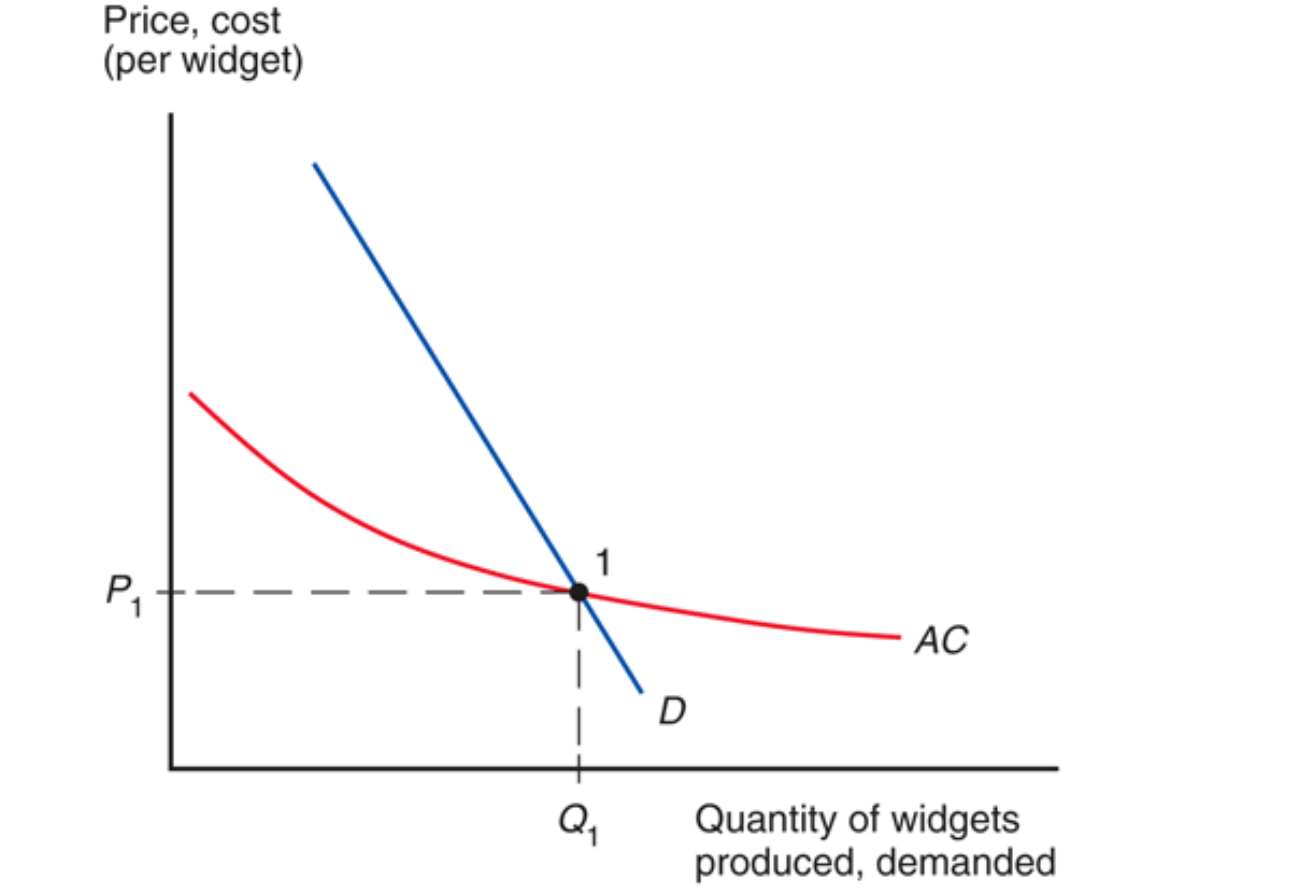
\includegraphics[scale=0.20]{ext_equil.png}
    \begin{itemize}
        \item Where does demand curve come from?
    \end{itemize}

\end{frame}

\begin{frame}{Pause}

    \begin{itemize}
        \item Simple 1 x 1 x 1 model
        \item Now add second country
        \item How does trade affect price?
    \end{itemize}

\end{frame}

\begin{frame}{Trade and External Economies}

    \begin{itemize}
        \item Two countries: China and US
        \item Two goods: Buttons and Not-Buttons
        \item One factor: Labor
        \item External economies of scale
    \end{itemize}

\end{frame}

\begin{frame}{No button trade}

    \begin{itemize}
        \item Each country makes its own buttons (and not-buttons)
    \end{itemize}
    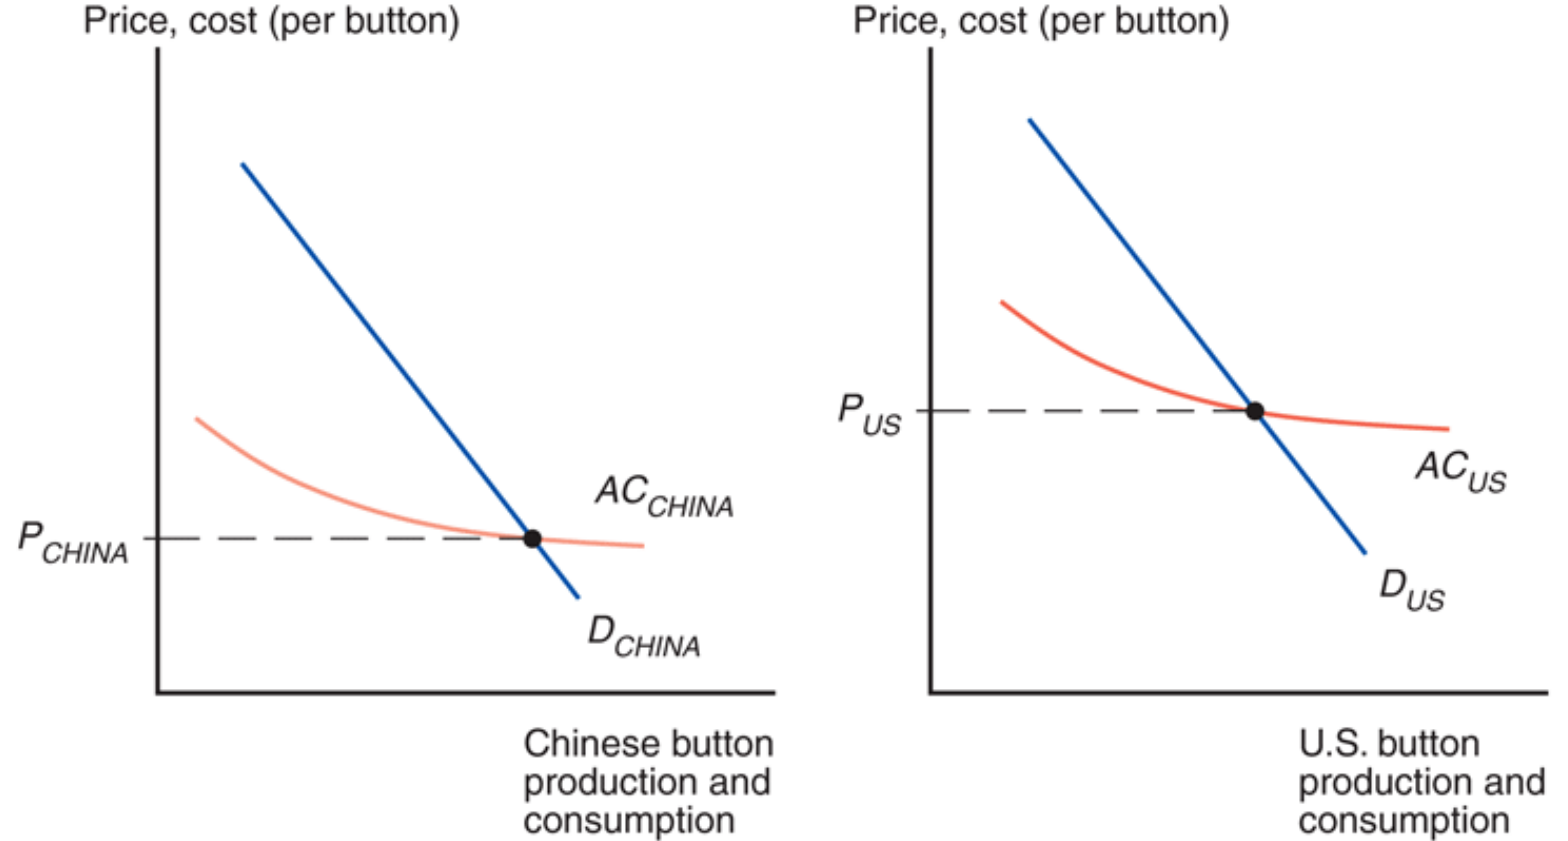
\includegraphics[scale=0.20]{buttons_aut.png}

\end{frame}

\begin{frame}{Allow button trade}

    \begin{itemize}
        \item Opening to trade
        \begin{itemize}
            \item China can undercut all American button makers 
            \item True even if very little Labor in American button making
            \item Increasing marginal product of labor (unlike other models)
            \item China makes all the buttons
        \end{itemize} 
        \item Scale economies
        \begin{itemize}
            \item Cost of producing buttons in China goes down
            \item Cost of producing buttons in US goes up 
            \item Cheaper buttons everywhere!
            \item What about real wages of Chinese workers?
            \item What about real wages of American workers?
        \end{itemize}
    \end{itemize}

\end{frame}

\begin{frame}{Allow button trade}

    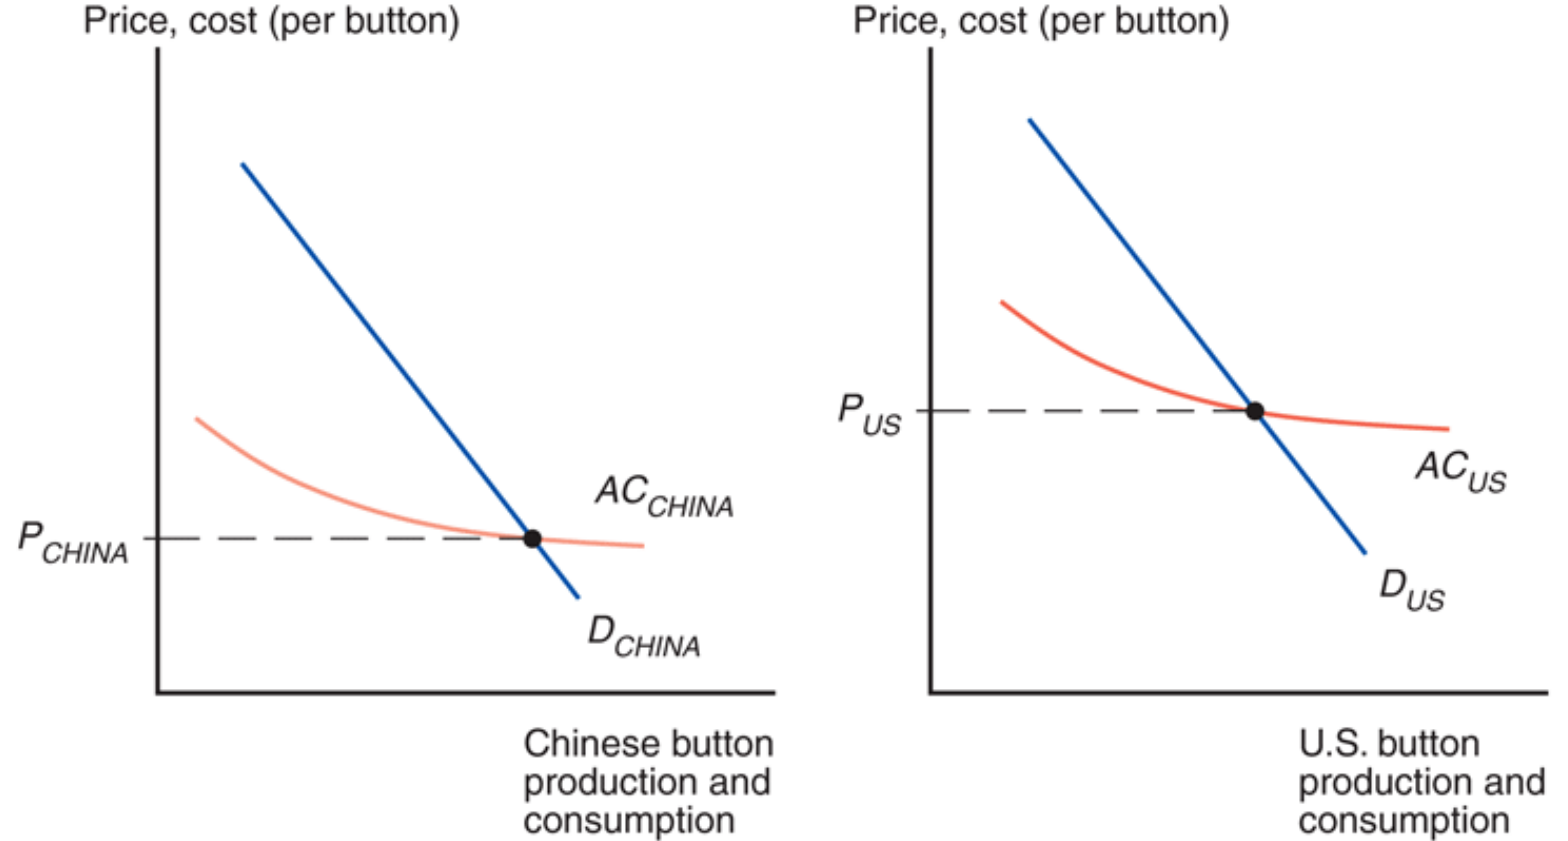
\includegraphics[scale=0.20]{buttons_aut.png}

\end{frame}

\end{document}






